\chapter{Introdução à Linguagem JavaScript}\label{cap:javaScript}
\epigraph{``\textit{A vida vai ficando cada vez mais dura perto do topo}''.}{Friedrich Nietzsche}

\lettrine[lines=4, lhang=0.1, lraise=0, loversize=0.2, findent=0.1em]{\textcolor{corAzulTema}{N}}{ESTE} Capítulo temos como objetivo aprender as construções básicas da linguagem de programação JavaScript, vastamente utilizada no desenvolvimento de aplicações Web.

\section{Introdução}

Chegamos a talvez à cereja do bolo, ou à cereja do livro ou então à cereja do desenvolvimento para Web: a linguagem de \textit{script} JavaScript. A primeira coisa que precisamos deixar claro é que Java e JavaScript são duas linguagens diferentes, com sintaxe baseada em C e com construções similares, mas o comum entre as duas para por aqui. A linguagem JavaScript não é uma linguagem orientada a objetos, mas sim baseada em protótipos. Nesse tipo de linguagem não existem classes, mas apenas objetos. Novos objetos são criados a partir de cópias de objetos existentes. O JavaScript ``moderno'', baseado no padrão ECMAScript 2015 (sexta edição), possui algumas construções que lembram àquelas de linguagens orientadas a objetos como classes e herança, mas tudo isso é \textit{syntax sugar} para simplificar coisas que já existiam anteriormente. Outras construções também são suportadas na linguagem como as funções de primeira classe etc.

Neste Capítulo não entraremos em detalhes sobre a história da linguagem e da sua evolução, mas sim no que eu acho útil e fundamental para que possamos começar a usá-la. Iremos ter uma visão geral da linguagem como declaração de variáveis, manipulação do \textit{Document Object Model} (DOM) e requisições assíncronas. Durante o Capítulo serão apresentadas inúmeras caixas do tipo ``Saiba Mais'' com \textit{links} úteis. A maioria desses links serão da \textit{Mozilla Developer Network}\footnote{\url{https://developer.mozilla.org/}} (MDN), uma referência confiável e oficial da maioria, senão de todas, das tecnologias para Web. Sempre fornecerei os \textit{links} da versão em inglês do site, mas se quiser, você pode verificar a versão em português clicando no botão ``\textit{Change language}'' presente em todas as páginas do site. Sinceramente recomendo a leitura em inglês, pois o texto sempre estará completo, atualizado com a terminologia correta.

\begin{saibaMais}
    Quer conhecer um pouco mais da história e dos detalhes da linguagem JavaScript? Veja o \textit{link} \url{https://developer.mozilla.org/en-US/docs/Web/JavaScript}.
\end{saibaMais}

\begin{saibaMais}
    A referência da linguagem JavaScript pode ser acessada pelo \textit{link} \url{https://developer.mozilla.org/en-US/docs/Web/JavaScript/Reference}.
\end{saibaMais}

\begin{saibaMais}
    As documentações e referências das tecnologias e APIs usadas para o desenvolvimento para Web podem ser acessadas pelo \textit{link} \url{https://developer.mozilla.org/en-US/docs/Web/API}.
\end{saibaMais}

\begin{saibaMais}
    Caso deseje fazer um tutorial completo sobre a linguagem, recomendo o ótimo tutorial da própria MDN: \url{https://developer.mozilla.org/en-US/docs/Learn/JavaScript}.
\end{saibaMais}

Antes de começarmos a falar do JavaScript propriamente dito, vamos montar nosso palco, que é um projeto Java para Web. Neste Capítulo ainda faremos a construção dos projetos do zero, mas a partir do próximo focarei apenas nas novidades que serão apresentadas.

Vamos lá. Crie um projeto Java Web com o nome de ``ExemplosEmJavaScript'' da forma que tem feito até aqui. Os passos descritos a seguir são somente estruturais. Os respectivos códigos dos arquivos serão apresentados e explicados posteriormente. Sendo assim, no nó \destaque{\textit{Web Pages}} do projeto:

\begin{itemize}
    \item Remova o arquivo \texttt{index.html};
    \item Crie um JSP chamado \texttt{index.jsp};
    \item Crie uma pasta chamada \texttt{css};
    \item Crie uma pasta chamada \texttt{js} (JavaScript);
    \item Dentro da pasta \texttt{css} crie um arquivo CSS chamado \texttt{estilos.css};
    \item Dentro da pasta \texttt{js} crie 12 arquivos JavaScript, chamados \texttt{exemplo01.js}, \texttt{exemplo02.js}... \texttt{exemplo12.js};
    \item Em \destaque{\textit{Source Packages}} crie os pacotes \texttt{exemplosemjavascript.pojo} e\newline%
    \texttt{exemplosemjavascript.servlets};
    \item No pacote \texttt{exemplosemjavascript.pojo} crie uma classe chamada \texttt{Pessoa};
    \item No pacote \texttt{exemplosemjavascript.servlets} crie os Servlets \texttt{CalculaTabuadaServlet} e \texttt{ListagemPessoasServlet};
    \item Importe e insira no projeto a biblioteca \texttt{Jakarta EE Web 8 API};
    \item Clique com o botão direito do mouse no nó raiz do projeto e escolha o último item do menu de contexto, chamado \destaque{\textit{Properties}};
    \begin{itemize}
        \item Do lado esquerdo, em \destaque{\textit{Categories:}}, clique no item \destaque{CDNJS}, situado dentro do nó \destaque{\textit{JavaScript Libraries}};
        \item Do lado direito, clique no botão \destaque{\textit{Add}};
        \item No diálogo que abriu, intitulado \destaque{\textit{Add CDNJS Library}}, preencha o campo \destaque{\textit{Find:}} com ``\texttt{jquery}'' (sem as aspas) e clique em \destaque{\textit{Search}};
        \item Após a busca na \textit{Content Delivery Network} (CDN) aparecerão diversos componentes na \textit{Graphical User Interface} (GUI). Em \destaque{\textit{Libraries:}} escolha \texttt{jquery}, provavelmente o primeiro item;
        \item Em \destaque{\textit{Files:}} marque a \textit{checkbox} na frente do item \texttt{jquery.min.js} e clique em \destaque{\textit{Add Library}} como na Figura~\ref{fig:cap07AddCDNJSLibrary};
        \FloatBarrier
        \begin{figure}[!htbp]
            \centering
            \caption{Adicionando uma biblioteca JavaScript}
            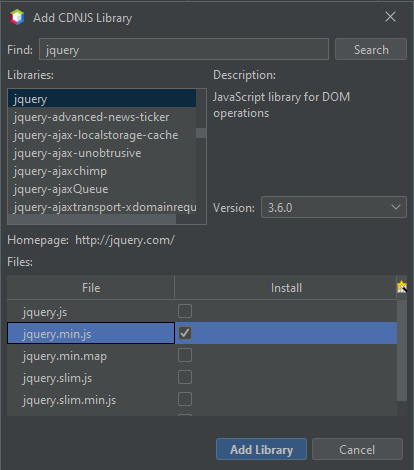
\includegraphics[scale=0.7]{imagens/cap07AddCDNJSLibrary}
            \\\textbf{Fonte:} Elaborada pelo autor
            \label{fig:cap07AddCDNJSLibrary}
        \end{figure}
        \FloatBarrier
        \item Clique em \destaque{OK}. A biblioteca jQuery será baixada e inserida no projeto dentro da pasta \texttt{js/libs/jquery}.
    \end{itemize}
\end{itemize}

Realizando todos os passos descritos anteriormente, você terá um projeto com a estrutura apresentada na Figura~\ref{fig:cap07EstruturaDoProjeto}. Agora vamos começar a preencher cada um dos arquivos e aprender o que está acontecendo em cada um deles.

\FloatBarrier
\begin{figure}[!htbp]
    \centering
    \caption{Estrutura do projeto}
    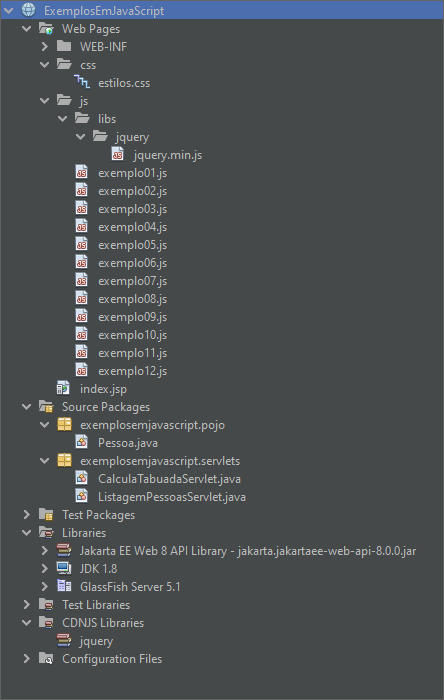
\includegraphics[scale=0.7]{imagens/cap07EstruturaDoProjeto}
    \\\textbf{Fonte:} Elaborada pelo autor
    \label{fig:cap07EstruturaDoProjeto}
\end{figure}
\FloatBarrier

Começaremos com o \texttt{index.jsp} apresentado na Listagem~\thechapter.\ref{listagem:projetos/capitulo07/ExemplosEmJavaScript/web/index.jsp}. Entre as linhas 10 e 22 usamos a \textit{tag} \inlineHTMLCode{<script>} para carregarmos no documento treze arquivos de código JavaScript. Inclusive, essa mesma \textit{tag} pode ser utilizada para inserir código JavaScript no próprio documento. Veremos isso mais adiante. Na linha 10 é carregada a biblioteca jQuery que há alguns anos atrás era absolutamente relevante, mas que hoje em dia tem caído em desuso visto a evolução do JavaScript. Ela será tratada no livro pela sua importância em software legado, por facilitar e padronizar algumas coisas e também, é claro, por preferência minha :D. No restante das linhas são associados os arquivos com os exemplos que aprenderemos. O restante do documento consiste na construção de uma GUI com alguns componentes e \textit{tags} que serão manipulados pelo nosso código em JavaScript. 

Os cinco primeiros exemplos são relativos às construções principais da linguagem. Veja que da linha 30 à 34 temos um parágrafo (\textit{tag} \inlineHTMLCode{<p>}) com um botão dentro (\textit{tag} \inlineHTMLCode{<button>}) e que em seu evento \textit{click}, representado pelo atributo \texttt{onclick}, é registrado uma função tratadora/manipuladora/ouvinte de evento (\textit{event handler} ou \textit{event listener}). Para registrar uma função como tratadora de um determinado evento, basta inserir seu nome no valor do atributo \texttt{onclick} e adicionar, entre os parânteses da mesma, a palavra \texttt{event}. Esse \texttt{event} carregará o objeto do evento que será disparado pela \textit{tag} e ouvido pela função. Essa função precisa estar declarada e implementada em algum lugar. No nosso caso, estará no arquivo \texttt{exemplo01.js}, referenciado acima. Note que como o JavaScript é interpretado, para se poder usar algo, essa ``coisa'' precisa ter sido declarada antes ou as vezes ``vista'' pelo interpretador pela primeira vez, sendo que esse segundo comportamento pode gerar muitos problemas caso não seja entendido apropriadamente, mas veremos isso também. Resumindo, ao se clicar (\texttt{onclick}) nesse primeiro botão, afunção \inlineJavaScriptCode{executarExemplo01(event)} será invocada. Fácil não é? Existe uma infinidade de eventos permitidos para cada \textit{tag}, mas falaremos de alguns deles à medida que for necessário. Esse padrão de um botão invocando uma função se repetirá em praticamente todos os exemplos. Os cinco primeiros têm a mesma estrutura.

Nos exemplos 06, 07 e 08 trataremos da manipulação das \textit{tags}, como dinamicamente inserir conteúdo nas mesmas ou ler/escrever dados em componentes de formulário. Esses exemplos estão dentro da seção ``Manipulação do DOM'', onde DOM significa \textit{Document Object Mode}l que nos bastidores é uma árvore composta de objetos que representam o resultado do processo de \textit{parsing} do arquivo HTML pelo navegador ou outro tipo de cliente. Usando JavaScript podemos mexer nessa árvore, alterando atributos dos nós, que na maioria das vezes representam as \textit{tags}, além de inserir e remover nós. Todas as modificações são replicadas automaticamente pelo navegador que entende que a árvore foi alterada e precisa ser redesenhada no processo de renderização do documento. Antigamente, quando isso era novidade há mais de 20 anos, era chamado de ``HTML Dinâmico'' (\textit{Dynamic} HTML (DHTML)). Sim, estou ficando velho :D. Perceba que nesses exemplos, além dos botões temos \textit{divs} que serão usadas para mostrar o resultado de algum processamento, além de componentes de formulário e outros botões no exemplo 08.

No exemplo 09 falaremos um pouco de tratamento de eventos, como já comentei anteriormente. Nesse exemplo, na linha 171, temos a invocação da função\newline%
\inlineJavaScriptCode{registrarEventosExemplo09()} em que, programaticamente, faremos o registro dos ouvintes de eventos ao invés de usar os atributos prefixados com ``\texttt{on}'' das \textit{tags}.

No exemplo 10 trataremos do uso da \textit{tag} \inlineHTMLCode{<canvas>} usada para desenhar programaticamente, realizando uma simulação física de uma bolinha.

Nos dois últimos exemplos trataremos das requisições assíncronas e de intercâmbio de dados entre cliente e servidor.

\htmlCode{Página principal da aplicação\newline%
Arquivo: \texttt{/index.jsp}}{projetos/capitulo07/ExemplosEmJavaScript/web/index.jsp}

Caso queira, durante os testes de execução, comente trechos do código do \texttt{index.jsp} para que você não precise ficar rolando a página para chegar em alguma parte toda vez que for testar uma funcionalidade.

Na Listagem~\thechapter.\ref{listagem:projetos/capitulo07/ExemplosEmJavaScript/web/css/estilos.css} é apresentado o arquivo com as folhas de estilo usadas no \texttt{index.jsp}. O código já contém os comentários para você entender o que se trata cada coisa.

\cssCode{Folhas de estilo do projeto\newline%
Arquivo: \texttt{/index.jsp}}{projetos/capitulo07/ExemplosEmJavaScript/web/css/estilos.css}

\begin{saibaMais}
    Sobre CSS, consulte \url{https://developer.mozilla.org/en-US/docs/Web/CSS} e \url{https://developer.mozilla.org/en-US/docs/Web/CSS/Reference}.
\end{saibaMais}

Nas próximas três listagens serão mostrados os componentes do lado do servidor que utilizaremos para os dois últimos exemplos. Na Listagem~\thechapter.\ref{listagem:projetos/capitulo07/ExemplosEmJavaScript/src/java/exemplosemjavascript/pojo/Pessoa.java} definimos a classe \texttt{Pessoa}, um \textit{Plain Old Java Object} (POJO) ou \textit{Value Object} (VO) que é uma classe que utilizaremos para criar objetos para transportar dados.

\javaCode{Classe Pessoa\newline%
Arquivo: \texttt{exemplosemjavascript/pojo/Pessoa.java}}{projetos/capitulo07/ExemplosEmJavaScript/src/java/exemplosemjavascript/pojo/Pessoa.java}

Na Listagem~\thechapter.\ref{listagem:projetos/capitulo07/ExemplosEmJavaScript/src/java/exemplosemjavascript/servlets/CalculaTabuadaServlet.java} é apresentado o código do Servlet \texttt{CalculaTabuadaServlet}, mapeado em \texttt{/calcularTabuada} que recebe um valor inteiro e retorna o texto representando a ``tabuada'' do número processado. Esse retorno é gerado pelo próprio Servlet no seu fluxo de saída (linhas 41, 42 e 43), sendo que o objeto response é configurado para indicar ao cliente que o que está chegando é no formato de texto/html (linha 28).

\javaCode{Servlet de tabuada\newline%
Arquivo: \texttt{exemplosemjavascript/servlets/CalculaTabuadaServlet.java}}{projetos/capitulo07/ExemplosEmJavaScript/src/java/exemplosemjavascript/servlets/CalculaTabuadaServlet.java}

Por fim, na Listagem~\thechapter.\ref{listagem:projetos/capitulo07/ExemplosEmJavaScript/src/java/exemplosemjavascript/servlets/ListagemPessoasServlet.java} é apresentado o código do Servlet \texttt{ListagemPessoasServlet}, mapeado em \texttt{/listarPessoas} que indica ao cliente que os dados que serão retornados irão no formato JavaScript Object Notation\footnote{O formato JSON será tratado no exemplo 05. Por enquanto assuma que é uma forma de codificar os dados de um objeto em forma de texto.} (JSON) (linha 33). Nesse Servlet é criada uma lista de objetos do tipo \texttt{Pessoa}, baseada na quantidade recebida via requisição e essa lista é serializada em JSON usando a camada de \textit{bindind} JSON-B do Java/Jakarta EE. Na linha 35 é criado o objeto serializador e na linha 56 ele é usado, convertendo a lista com os objetos do tipo \texttt{Pessoa} em uma representação em texto, que no nosso caso é o JSON.

\javaCode{Servlet de listagem de pessoas usando JSON\newline%
Arquivo: \texttt{exemplosemjavascript/servlets/ListagemPessoasServlet.java}}{projetos/capitulo07/ExemplosEmJavaScript/src/java/exemplosemjavascript/servlets/ListagemPessoasServlet.java}

Agora que temos toda a infraestrutura básica do nosso projeto, podemos começar a falar sobre JavaScript. Vamos começar!



\section{Funções de E/S e Operadores Aritméticos}

Começaremos nossa breve jornada de descoberta da linguagem JavaScript aprendendo uma forma de obter dados do usuário, que normalmente não é usada em um software em produção, mas para aprender conceitos vai nos servir no momento, como gerar saída, declarar variáveis e realizar as operações aritméticas básicas. Na Listagem~\thechapter.\ref{listagem:projetos/capitulo07/ExemplosEmJavaScript/web/js/exemplo01.js} pode ser visto o código completo do primeiro exemplo. Veja que logo na primeira linha há a declaração da função \inlineJavaScriptCode{executarExemplo01(event)} que é a função que tratará o evento \texttt{click} do primeiro botão do \texttt{index.jsp}.

\javaScriptCode{Exemplo 01\newline%
Arquivo: \texttt{/js/exemplo01.js}}{projetos/capitulo07/ExemplosEmJavaScript/web/js/exemplo01.js}

Na linha 5 é declarada uma variável local usando a palavra chave \inlineJavaScriptCode{let}\footnote{Veremos o propósito da palavra chave \texttt{let} no exemplo 02.}, com o identificador \inlineJavaScriptCode{n1} e atribuímos a ela o retorno da função \inlineJavaScriptCode{prompt}. Essa função recebe como parâmetro uma String e, ao ser executada, apresenta ao usuário um diálogo com uma mensagem (a String passada), um campo de texto, um botão de confirmação e um de cancelamento. Ao se clicar no botão de confirmação o valor fornecido do campo de texto será retornado ao chamador, no caso, atribuído à variável \inlineJavaScriptCode{n1} e se o diálogo for cancelado, será retornado o valor \inlineJavaScriptCode{null}. O retorno, quando válido, é do tipo String. Note que não declaramos o tipo das variáveis em JavaScript, pois a tipagem das variáveis é dinâmica, visto que o tipo de cada variável depende do valor atribuído ou referenciado por ela.

Na linha 9 fazemos basicamente a mesma coisa para a variável \inlineJavaScriptCode{n2}, mas o retorno da função \inlineJavaScriptCode{prompt} é usada como argumento da função \inlineJavaScriptCode{Number} que converterá a String retornada por \inlineJavaScriptCode{prompt} em um número e então esse valor será atribuído a \inlineJavaScriptCode{n2}.

Entre as linhas 12 e 16 declaramos cinco novas variáveis e atribuímos a elas o resultado de cinco operações. Note que como \inlineJavaScriptCode{n1} referencia uma String, o operador \inlineJavaScriptCode{+} será tratado como operador de concatenação de Strings ao invés de adição, ou seja, \inlineJavaScriptCode{n2} será convertida para String e concatenada com \inlineJavaScriptCode{n1}! Como os outros operadores como são aplicáveis apenas à números, \inlineJavaScriptCode{n1} será convertido implicitamente e a operação será realizada. O resultado disso será visto na saída que será gerada e exibida.

Falando da saída, na linha 19 declaramos a variável \inlineJavaScriptCode{saida} e concatenamos diversas Strings para gerar o resultado. Em JavaScript existem três literais para Strings:
  
\begin{enumerate}
    \item Delimitadas por aspas simples (apóstrofo): \inlineJavaScriptCode{'uma string'};
    \item Delimitadas por aspas duplas (aspas): \inlineJavaScriptCode{"outra string"};
    \item Delimitadas por acento grave (crase): \inlineJavaScriptCode{`mais uma string`};
\end{enumerate}

Os dois primeiros são análogos, com a diferença que quando se usa aspas simples como delimitador e queremos ter uma aspas simples dentro da String, precisamos escapá-la com contrabarra (barra invertida) e as aspas duplas não precisam. Por exemplo, \inlineJavaScriptCode{'a\'b"c'} corresponde à \destaque{\texttt{a\textquotesingle{}b"c}}. Quando delimitamos a String com aspas duplas temos o contrário, ou seja, \inlineJavaScriptCode{"a'b\"c"} correspondendo à \destaque{\texttt{a\textquotesingle{}b"c}}.

O terceiro tipo de delimitador é mais interessante, pois permite que façamos a interpolação de valores dentro da String usando uma notação parecida com a da EL do Java/Jakarta EE, mas que não tem relação a não ser a sintaxe similar. Para o nosso exemplo, se \inlineJavaScriptCode{n1} valer \inlineJavaScriptCode{"10"} e \inlineJavaScriptCode{n2} valer \inlineJavaScriptCode{5}, o resultado de \inlineJavaScriptCode{`${n1} e ${n2}`} será \destaque{\texttt{10 e 5}}.

Por fim, para apresentar a String gerada, usamos duas formas. A primeira, na linha 29, com a função \inlineJavaScriptCode{alert} que, assim como \inlineJavaScriptCode{prompt}, é bloqueante, fazendo a execução do código parar naquele ponto ao esperar a interação do usuário. Essa função recebe uma String como parâmetro e a mostra num diálogo ao ser executada. A outra forma é usando a função \inlineJavaScriptCode{log} do objeto \inlineJavaScriptCode{console}, que recebe um ou vários objetos como parâmetro e os mostram no console do navegador. No nosso exemplo, a exibição no console está condicionada ao retorno da função \inlineJavaScriptCode{confirm} que exibe uma mensagem ao usuário e aguarda a interação. Caso o usuário confirme a mensagem, a função retornará um valor verdadeiro, usado na estrutura condicional \inlineJavaScriptCode{if} do exemplo.



\section{Declarações de Variáveis e Suas Implicações}

Como já dito, as variáveis em JavaScript não tem um tipo definido, visto que a linguagem é dinamicamente tipada, implicando que o tipo da variável varia de acordo com o que ela referencia. Em JavaScript temos Strings, números, valores lógicos, funções, objetos entre outros.

Toda variável em JavaScript ao ser declarada passará pelo processo de \textit{hoisting}. Nesse processo, a variável será elevada ou içada até o início ou topo do contexto em que ela foi declarada e que passará a existir. A ideia é que quando o interpretador encontra uma declaração de variável e ela é bem sucedida, ou seja, é válida sintática e semanticamente, ela passará a existir como se houvesse sido declarada no início do escopo em que reside.

Podemos influenciar em como a inicialização das variáveis será feita. Veja a lista abaixo, temos quatro formas de declarar variáveis:

\begin{enumerate}
    \item \inlineJavaScriptCode{let variavel = "valor";};
    \item \inlineJavaScriptCode{const constante = "valor";};
    \item \inlineJavaScriptCode{var variavel = "valor";};
    \item \inlineJavaScriptCode{variavel = "valor";};
\end{enumerate}

Quando a palavra-chave \inlineJavaScriptCode{let} é usada, a variável só poderá ser usada depois da sua inicialização, mesmo havendo \textit{hoisting} para ela. O mesmo acontece com as constantes, declaradas com \inlineJavaScriptCode{const}. Já as variáveis declaradas com a palavra-chave \inlineJavaScriptCode{var} serão inicializadas com \inlineJavaScriptCode{undefined}. Por fim, as variáveis que são declaradas sem indicar nenhuma dessas três palavras-chave passarão a existir no escopo global, o que pode trazer uma série de problemas. Imagine que você declarou mais de uma variável com o mesmo nome em dois ou mais escopos diferentes. A declaração de fato ocorrerá quando o interpretador a encontrar pela primeira vez e, independende de onde for, ela passará a existir no escopo global e a partir desse ponto você pode perder o controle do valor que a variável referencia se não tomar muito cuidado com o que está fazendo. O ideal é não utilizar ok?

O exemplo apresentado na Listagem~\thechapter.\ref{listagem:projetos/capitulo07/ExemplosEmJavaScript/web/js/exemplo02.js} mostra todos esses efeitos quando for executado. O ``problema'' da variável declarada sem \inlineJavaScriptCode{let}, \inlineJavaScriptCode{var} ou \inlineJavaScriptCode{const} pode ser reproduzido ao se clicar pela segunda vez no botão do exemplo 02.

\javaScriptCode{Exemplo 02\newline%
Arquivo: \texttt{/js/exemplo02.js}}{projetos/capitulo07/ExemplosEmJavaScript/web/js/exemplo02.js}

Veja o exemplo, todo o código está comentado, não sendo necessário entrar em mais detalhes. Recomendo que você dê uma olhada nos \textit{links} disponibilizados nas próximas duas caixas ``Saiba Mais''.

\begin{saibaMais}
    Para uma explicação mais detalhada sobre essas implicações, acesse \url{http://www.constletvar.com/}.
\end{saibaMais}

\begin{saibaMais}
    Para mais detalhes sobre declaração de variáveis em JavaScript, acesse \url{https://developer.mozilla.org/en-US/docs/Web/JavaScript/Reference/Statements}.
\end{saibaMais}

Esse conceito pode gerar muita confusão, inclusive se declararmos uma variável com \inlineJavaScriptCode{var} no contexto global (fora de funções) ela será uma variável global (uma propriedade do objeto \texttt{window}), ao passo que dentro de uma função ela terá escopo local, assim como \inlineJavaScriptCode{let} e \inlineJavaScriptCode{const}, mas inicializada como \inlineJavaScriptCode{undefined}. Ainda, é importante frisar que uma constante tem ligação imutável (\textit{immutable binding}) com o que ela referencia, ou seja, ela não pode receber um novo valor, mas o objeto que ela referencia pode ser modificado (ele não é imutável).



\section{Estruturas Condicionais e Operadores}

Em JavaScript temos as mesmas estruturas condicionais presentes na maioria das linguagens de programação ou seja, um \inlineJavaScriptCode{if} com \inlineJavaScriptCode{else}s aninhados e opcionais e um \inlineJavaScriptCode{switch}. Os operadores relacionais e lógicos também são os operadores padrão encontrados na maioria das linguages derivadas de C, com a adição de mais dois operadores relacionais que são o operador de identidade (\inlineJavaScriptCode{===}) e o operador de não identidade (\inlineJavaScriptCode{!==}). Ao passo que os operadores de igualdade e de desigualdade verificam se o valor dos operandos comparados são respectivamente iguais ou difentes, inclusive após a conversão implícita de algum deles, os operadores de identidade e de não identidade verificam, além do valor (sem conversão implícita), respectivamente, se o tipo é o mesmo ou diferente. Na Listagem~\thechapter.\ref{listagem:projetos/capitulo07/ExemplosEmJavaScript/web/js/exemplo03.js} pode ser visto o emprego das estruturas condicionais e a declaração de variáveis com alguns valores permitidos.

\javaScriptCode{Exemplo 03\newline%
Arquivo: \texttt{/js/exemplo03.js}}{projetos/capitulo07/ExemplosEmJavaScript/web/js/exemplo03.js}

\begin{saibaMais}
    Para mais detalhes sobre os operadores em JavaScript, acesse \url{https://developer.mozilla.org/en-US/docs/Web/JavaScript/Reference/Operators}.
\end{saibaMais}


\section{Estruturas de Repetição e Arrays}

Os Arrays em JavaScript atuam como arrays na linguagem Java e C, sendo indexados iniciando em 0, mas podendo crescer ou diminuir quando necessário, assemelhando-se mais com listas do que arrays de tamanho fixo. Podemos usar a notação de colchetes para ``simular'' arrays associativos (tabelas de símbolos), mas de fato o que acontece é que estamos criando ou lendo propriedades do objeto do array. Na Listagem~\thechapter.\ref{listagem:projetos/capitulo07/ExemplosEmJavaScript/web/js/exemplo04.js} pode se ver a criação de três arrays e a utilização da estrutura de repetição \inlineJavaScriptCode{for} para iterar por seus elementos.

\javaScriptCode{Exemplo 04\newline%
Arquivo: \texttt{/js/exemplo04.js}}{projetos/capitulo07/ExemplosEmJavaScript/web/js/exemplo04.js}

Na linha 4 um array de uma dimensão é criado e inicializado com os valores 1, 2, 3 e 4, contidos respectivamente nas posições 0, 1, 2 e 3. Na linha 7 é criado um array em que nas posições 0 e 1 estão contidos dois outros arrays, um com os valores 1 e 2 e o outro com os valores 3 e 4.

Na linha 10 um novo array vazio é criado e entre as linhas 11 e 14 são inseridas quatro propriedades no objeto em si. Note que essas propriedades são criadas no objeto e pela sintaxe usada, há a impressão que estamos lidando com o array como se fosse um array associativo ou uma tabela de símbolos, mapa ou dicionário, mas não é o caso! Podemos usar a notação de colchetes para lidar com objetos para, por exemplo, acessar propriedades ou atributos que contenham espaço nos nomes. Note que posteriomente, ao se tentar iterar por esse array usando um \inlineJavaScriptCode{for} ``normal'', não se entrará no bloco da estrutura de repetição, visto que, apesar de parecer que o array contém quatro elementos, na verdade ele não tem nenhum, fazendo com que o atributo \inlineJavaScriptCode{length} valha zero.

A inserção e remoção de elementos dos arrays podem ser feitas usando os métodos \inlineJavaScriptCode{push} que insere um elemento no fim do array, \inlineJavaScriptCode{pop} que remove um elemento do fim, \inlineJavaScriptCode{unshift} que insere um elemento no início, \inlineJavaScriptCode{shift} que remove do início e \inlineJavaScriptCode{splice} que remove de uma posição arbitrária. Na caixa ``Saiba Mais'' abaixo você pode dar uma olhada na documentação do objeto Array da linguagem JavaScript.

\begin{saibaMais}
    Para mais detalhes sobre o tipo Array em JavaScript, acesse \url{https://developer.mozilla.org/en-US/docs/Web/JavaScript/Reference/Global_Objects/Array}.
\end{saibaMais}

Entre as linhas 24 e 26 usa-se um \inlineJavaScriptCode{for} para iterar pelos elementos do array \inlineJavaScriptCode{a1}. Entre as linhas 30 e 32 usa-se o método \inlineJavaScriptCode{forEach} do objeto Array para iterar pelos elementos, usando uma função de \textit{callback} para processar cada posição. A mesma coisa acontece entre as linhas 34 e 41, com a diferença de se usar a notação de \textit{closure} para a definição da função de \textit{callback} utilizada no método \inlineJavaScriptCode{forEach} de \inlineJavaScriptCode{a2}.

Como mencionado anteriormente, o uso de um \inlineJavaScriptCode{for} padrão -ou mesmo um \inlineJavaScriptCode{forEach}- para \inlineJavaScriptCode{a3} não surtirá efeito, pois esse array está vazio! Nós inserimos quatro propriedades no mesmo, não quatro elementos. Quando usamos um array dessa forma, inclusive poderia ser qualquer objeto, e queremos iterar por essas propriedades temos basicamente duas formas: ou fazemos como entre as linhas 58 e 60, usando um \inlineJavaScriptCode{for ... in} ou obtemos as chaves do objeto como um array e as processamos usando um \inlineJavaScriptCode{forEach} como mostrado entre as linhas 63 e 65.

Além do método \inlineJavaScriptCode{forEach} existem alguns outros para o processamento dos elementos de um array. Dois desses métodos são mostrados a partir da linha 80: \inlineJavaScriptCode{every} e \inlineJavaScriptCode{some}. Como os nomes sugerem, o primeiro é utilizado com a premissa de testar alguma condição em todos os elementos do array, enquanto o outro espera-se que algum elemento não se enquadre em algo desejado. Podemos utilizar esses métodos para, por exemplo, executar uma busca/pesquisa sequencial/linear no array e parar a iteração quando o elemento for encontrado, retornando um valor verdadeiro ou falso, dependendo da situação e do método empregado. Veja os comentários do exemplo e teste a execução do código para entender exatamente do que se trata.



\section{``Classes'', Objetos e JSON}

Antes do ECMAScript 2015 (sexta edição) a criação de objetos com um ``tipo'' era feito a partir do uso de uma função e o operador \inlineJavaScriptCode{new}. A partir do ECMAScript 2015 existe uma sintaxe para a definição de tipos abstratos de dados em forma de classes, inclusive permitindo herança entre os tipos definidos. Na Listagem~\thechapter.\ref{listagem:projetos/capitulo07/ExemplosEmJavaScript/web/js/exemplo05.js}, entre as linhas 1 e 17 é definida a classe \texttt{Forma}. As classes em JavaScript podem ter apenas um construtor e, dentro dele, as propriedades do objeto devem ser criadas utilizando a palavra chave \inlineJavaScriptCode{this}.

\javaScriptCode{Exemplo 05\newline%
Arquivo: \texttt{/js/exemplo05.js}}{projetos/capitulo07/ExemplosEmJavaScript/web/js/exemplo05.js}

Entre as linhas 20 e 43 são declaradas as classes \texttt{Retangulo} e \texttt{Circulo} que herdam de \texttt{Forma}, sobrescrevendo o método \inlineJavaScriptCode{calcularArea()}. Nas linhas 47 e 48 cria-se respectivamente uma instância de \texttt{Retangulo} e uma de \texttt{Circulo}. Entre as linhas 51 e 66 cria-se um novo objeto genérico, usando o inicializador de objetos (abre e fecha chaves). Note que esse objeto e os outros dois tem como tipo \texttt{object} (linhas 69 a 71), mas é possível verificar se são instância de uma determinada classe/tipo usando o operador \inlineJavaScriptCode{instanceof} como visto entre as linhas 74 e 87.

Podemos também representar objetos inteiros como Strings usando a notação de objetos JavaScript, chamada de JSON. Veja na linha 91 onde temos uma String codificando um objeto usando algo similar à notação de inicilização de objetos. Isso é o JSON. Para transformar essa String em um objeto, usa-se o método \inlineJavaScriptCode{parse()} do objeto global \inlineJavaScriptCode{JSON} e, quando se quer o contrário, ou seja, transformar um objeto em uma String no formato JSON, usa-se o método \inlineJavaScriptCode{stringfy()} também do objeto \inlineJavaScriptCode{JSON}. O formato JSON é amplamanete utilizado atualmente em detrimento do formado XML, pois é mais enxuto, ou seja, é necessário menos texto para codificar o mesmo objeto em JSON do que em XML. Tanto o formato JSON quanto XML são utilizados para a serialização de objetos, ou seja, transformar uma representação binária, específica de linguagem, em uma representação serial fácil de ser processada e independente de plataforma. O processo de converter um objeto para um formato de intercâmbio de dados é chamado de serialização, enquanto o processo inverso, ou seja, a partir de um formato de intercâmbio de dados gerar um objeto específico de tecnologia é chamado de desserialização.

O restante do código do exemplo é facilmente entendido ao ser lido. Nas próximas caixas ``Saiba Mais'' há varios links úteis sobre o tema.

\begin{saibaMais}
    Para saber mais sobre classes em JavaScript, acesse \url{https://developer.mozilla.org/en-US/docs/Web/JavaScript/Reference/Classes}.
\end{saibaMais}

\begin{saibaMais}
    Para consultar a documentação sobre o tipo String em JavaScript, acesse \url{https://developer.mozilla.org/en-US/docs/Web/JavaScript/Reference/Global_Objects/String}.
\end{saibaMais}

\begin{saibaMais}
    Para consultar a documentação sobre JSON em JavaScript, acesse \url{https://developer.mozilla.org/en-US/docs/Web/JavaScript/Reference/Global_Objects/JSON}.
\end{saibaMais}



\section{Manipulação do DOM}

Nesta Seção aprenderemos a manipular o DOM com objetivo de extrair dados do documento ou então modificá-lo em tempo de execução. Isso já foi comentado brevemente.

\begin{saibaMais}
    A documentação do DOM pode ser vista no \textit{link} \url{https://developer.mozilla.org/en-US/docs/Web/API/Document_Object_Model}.
\end{saibaMais}

Vamos manipular o DOM de duas formas, uma usando JavaScript puro, que normalmente é mais verboso, e a outra usando a biblioteca jQuery\footnote{\url{https://jquery.com/}}, que já foi padrão na construção de aplicações para Web e tem caído em desuso, mas ainda é relevante, principalmente por facilitar algumas coisas e ainda estar presente de forma consistente em diversas aplicações criadas e que você provavelmente terá que dar manutenção na sua vida profissional.


\subsection{JavaScript Puro}

A ideia desse exemplo é que ao se clicar no botão, um novo nó da \textit{tag} \inlineHTMLCode{<p>} seja inserido na \inlineHTMLCode{<div>} que tem \texttt{id} igual à \texttt{divExemplo06}, usando um contador para mostrar as sucessivas inserções. Na linha 6 da Listagem~\thechapter.\ref{listagem:projetos/capitulo07/ExemplosEmJavaScript/web/js/exemplo06.js} obtém-se tal \inlineHTMLCode{<div>} utilizando o método \inlineJavaScriptCode{getElementById("id")} do objeto \inlineJavaScriptCode{document}. Caso bem-sucedido, o método retornará uma referência ao nó dessa \inlineHTMLCode{<div>} no DOM e então poderemos manipulá-lo! Na linha 9 criamos um novo nó para inserir na \inlineHTMLCode{<div>} do tipo correspondente à \textit{tag} \inlineHTMLCode{<p>}. Entre as linhas 12 e 13 inserimos o conteúdo do parágrafo criado e defimos qual é sua classe. Veja no arquivo \texttt{estilos.css} que temos a definição de um seletor de classe chamado \inlineCSSCode{.pDOM} que refletirá na inserção desses parágrafos, sendo que todo item par terá uma cor de fundo azulada. Por fim, na linha 16 esse novo parágrafo é inserido na \inlineHTMLCode{<div>} e essa alteração é prontamente refletida na renderização do documento! Pare e pense agora todas as possibilidades existentes!

\javaScriptCode{Exemplo 06\newline%
Arquivo: \texttt{/js/exemplo06.js}}{projetos/capitulo07/ExemplosEmJavaScript/web/js/exemplo06.js}


\subsection{Usando jQuery}

Talvez os dois principais diferenciais ou chamarizes da jQuery que a tornaram famosa é a utilização da sintaxe de seletores do CSS para obter elementos do DOM, o que já foi implementado de forma nativa no JavaScript através de função \inlineJavaScriptCode{querySelector} do objeto \inlineJavaScriptCode{document} e a facilidade para lidar com requisições assíncronas com o servidor, o que também já foi endereçado nas versões mais novas do JavaScript.

No exemplo apresentado na Listagem~\thechapter.\ref{listagem:projetos/capitulo07/ExemplosEmJavaScript/web/js/exemplo07.js} temos algo análogo ao exemplo anterior, só que usando as funcionalidades dessa biblioteca. Na linha 7 obtemos a \inlineHTMLCode{<div>} que tem \texttt{divExemplo07} como \texttt{id} usando a notação de seletores do CSS! As funcionalidades da jQuery são acessadas através do símbolo de cifrão (\texttt{\$}) que é um \textit{alias} (apelido) para o objeto chamado \texttt{jQuery}, disponível para ser utilizado nos \textit{scripts} a partir do momento em que a biblioteca é inserida no documento. A criação do parágrafo também é mais direta, bastando inserir o par de \textit{tags} como String no argumento da função \texttt{\$} e então encadear a invocação dos métodos \inlineJavaScriptCode{html} e \inlineJavaScriptCode{addClass}. A linha 16 é idêntica ao exemplo anterior.

\javaScriptCode{Exemplo 07\newline%
Arquivo: \texttt{/js/exemplo07.js}}{projetos/capitulo07/ExemplosEmJavaScript/web/js/exemplo07.js}

\begin{saibaMais}
    Se quiser aprender um pouco mais sobre a jQuery, acesse \url{https://learn.jquery.com/}.
\end{saibaMais}

\begin{saibaMais}
    Sobre a função \inlineJavaScriptCode{querySelector}, acesse \url{https://developer.mozilla.org/pt-BR/docs/Web/API/Document/querySelector}.
\end{saibaMais}



\section{Manipulação de Formulários}

A ideia central presente neste Capítulo é fazer com que você entenda um pouco sobre JavaScript para podermos ter formulários mais sofisticados, permitindo a construção de cadastros que envolvam relacionamos muitos-para-muitos. Claro que estamos vendo várias coisas a mais, mas a ideia é dar subsídios para implementarmos coisas novas no projeto iniciado no Capítulo~\ref{cap:primeiroProjeto}. No exemplo apresentado na Listagem~\thechapter.\ref{listagem:projetos/capitulo07/ExemplosEmJavaScript/web/js/exemplo08.js} veremos a obtenção e a inserção de dados em componentes de formulários. Detalharei alguns pontos do código e, para não ficar muito maçante, o restante é com você. Tenho certeza que entenderá o que está acontecendo com base no que foi visto até agora.

\javaScriptCode{Exemplo 08\newline%
Arquivo: \texttt{/js/exemplo08.js}}{projetos/capitulo07/ExemplosEmJavaScript/web/js/exemplo08.js}

Neste exemplo são definidas seis funções que tratarão o evento \textit{click} de seis botões. A ideia é apresentar três situações de duas formas diferentes, uma com JavaScript puro e uma usando jQuery. Na linha 11 da primeira função, \inlineJavaScriptCode{lerDadosFormulario(event)}, obtemos o valor do campo de texto identificado por \texttt{campo01} em seu \texttt{id}. Veja que obtemos o elemento pelo \texttt{id} (método \inlineJavaScriptCode{getElementById( "id" )}), acessamos a propriedade \texttt{value} e atribuímos à variável \inlineJavaScriptCode{campo01}. Podemos também obter componentes pelo atributo \texttt{name}, entretanto pode haver mais de um componente com o mesmo \texttt{name}, então o método \inlineJavaScriptCode{getElementsByName( "name" )} retorna um array. No nosso exemplo há apenas um componente com o nome \texttt{campo02}, mas como o retorno do método \inlineJavaScriptCode{getElementsByName( "name" )} é um array, precisamos obter o primeiro elemento do array retornado e então obter o valor.

Entre as linhas 18 e 20 obtemos o valor de dois componentes \inlineHTMLCode{<select>} e um \inlineHTMLCode{<textarea>}. Note que para os \textit{selects} o valor retornado será o da opção selecionada no momento. Por fim, entre as linhas 22 e 27, apresentamos os valores lidos usando um alerta.

A segunda função implementada, \inlineJavaScriptCode{lerDadosFormularioJQuery(event)}, faz a mesma coisa que a primeira, entretanto usando jQuery. Perceba que o código fica mais limpo e enxuto. Basta usar o seletor de \texttt{id} do CSS para obter o componente desejado e usar o método \inlineJavaScriptCode{val()} para obter o valor.

O segundo conjunto de funções, \inlineJavaScriptCode{inserirDadosFormulario(event)} e \newline%
\inlineJavaScriptCode{inserirDadosFormularioJQuery(event)}, faz o processo inverso, ou seja, ao invés de ler os dados para fazer alguma coisa, os dados são inseridos nos componentes. Perceba que a definição da função \inlineJavaScriptCode{inserirDadosFormulario(event)} é feita usando a notação de \textit{closures}, atribuindo a função à variável \inlineJavaScriptCode{inserirDadosFormulario}.

Por fim, na última dupla de funções, \inlineJavaScriptCode{inserirNovaOpcao(event)} e \newline%
\inlineJavaScriptCode{inserirNovaOpcaoJQuery(event)} temos o exemplo de criar uma nova opção para os componentes \textit{select}. Isso será útil no nosso próximo projeto.



\section{Eventos}

Quase todas as \textit{tags} HTML disparam uma vasta quantidade de tipos de eventos que podem ser tratados. Claro que a maioria dos eventos ``úteis'' são ouvidos em componentes visíveis, mas há inúmeras possibilidades. Na Listagem~\thechapter.\ref{listagem:projetos/capitulo07/ExemplosEmJavaScript/web/js/exemplo09.js} é apresentado como se faz programaticamente o registro de tratadores de eventos em nós do DOM ao invés de fazer isso direto no HTML como estamos fazendo com os botões.

\javaScriptCode{Exemplo 09\newline%
Arquivo: \texttt{/js/exemplo09.js}}{projetos/capitulo07/ExemplosEmJavaScript/web/js/exemplo09.js}

É importante perceber que essa função precisa ser executada para que os tratadores de eventos sejam registrados de fato, sendo assim, na linha 171 da Listagem~\thechapter.\ref{listagem:projetos/capitulo07/ExemplosEmJavaScript/web/index.jsp}, essa função é invocada dentro da \textit{tag} \inlineHTMLCode{<script>}. Normalmente quando se quer registrar eventos programaticamente no documento isso é feito quando todo o documento está pronto para ser processado, ou seja, todo o DOM foi construído. Veremos isso na prática no Capítulo~\ref{cap:terceiroProjeto}.

Usando JavaScript puro, o registro de eventos é feito associando às propriedades prefixadas com \texttt{on} dos nós do DOM uma função para o tratamento dos mesmos. Na linha 4 da Listagem~\thechapter.\ref{listagem:projetos/capitulo07/ExemplosEmJavaScript/web/js/exemplo09.js} pode-se ver a obtenção de um campo de texto e o registro do tratador de evento para o evento ``key down'' (tecla pressionada) que mostrará, via \inlineJavaScriptCode{console.log(...)}, o caractere digitado no campo de texto.

Já na linha 9 fazemos o registro do evento \textit{change} de um \textit{select} usando jQuery. Veja como a sintaxe é diferente. O evento \textit{change} é disparado quando se seleciona uma opção do \textit{select} em questão, desde que a opção seja diferente da opção selecionada no momento. No nosso caso, o valor da opção selecionada será mostrada usando um alerta.

Na caixa ``Saiba Mais'' abaixo você poderá conferir uma lista completa de todos os eventos que existem e podem ser usados.

\begin{saibaMais}
    A documentação completa sobre os eventos que podem ser tratados pode ser vista em  \url{https://developer.mozilla.org/en-US/docs/Web/Events}.
\end{saibaMais}



\section{Simulação Usando a Canvas API}

Nesta Seção falaremos um pouco sobre o \textit{tag} \inlineHTMLCode{<canvas>} e sobre a Canvas API, que nos permitirá realizar operações de desenho em Duas Dimensões (2D). Atualmente, além de trabalhar com desenhos em duas dimensões, podemos também usar a WebGL API para realizar desenhos em 2D ou Três Dimensões (3D) usando aceleração em \textit{hardware}, mas isso foge demais do escopo deste livro. Focaremos no 2D realizando a simulação da física de ``bolinhas'' que serão animadas para que você possa conhecer um pouco sobre a Canvas API e sobre a utilização da função \inlineJavaScriptCode{setInterval(...)} que nos permetirá executar código repetidamente em um intervalo predefinido de tempo. Na Listagem~\thechapter.\ref{listagem:projetos/capitulo07/ExemplosEmJavaScript/web/js/exemplo10.js} podemos ver o código completo do exemplo.

\javaScriptCode{Exemplo 10\newline%
Arquivo: \texttt{/js/exemplo10.js}}{projetos/capitulo07/ExemplosEmJavaScript/web/js/exemplo10.js}

Entre as linhas 3 e 121 definimos uma classe chamada \texttt{Bolinha}. A ideia é que essa classe modele uma bolinha, na verdade um círculo pequeno, que estará suscetível à forças físicas que simularemos. O construtor da classe, iniciado na linha 6, possui seis parâmetros:

\begin{itemize}
    \item \inlineJavaScriptCode{x}: é a posição do centro da bolinha no eixo $x$;
    \item \inlineJavaScriptCode{y}: é a posição do centro da bolinha no eixo $y$;
    \item \inlineJavaScriptCode{velocidadeX}: é a quantidade de \textit{pixels} que a bolinha vai ser movida no eixo $x$ a cada passo da simulação;
    \item \inlineJavaScriptCode{velocidadeY}: é a quantidade de \textit{pixels} que a bolinha vai ser movida no eixo $y$ a cada passo da simulação;
    \item \inlineJavaScriptCode{raio}: representa o raio do círculo;
    \item \inlineJavaScriptCode{cor}: é a cor que será utilizada para desenhar a bolinha.
\end{itemize}

Ao construir a bolinha esses valores serão usados para inicializar os atributos correspondentes e, além desses, outros atributos serão criados com valores fixos:

\begin{itemize}
    \item \inlineJavaScriptCode{elasticidade}: representa algo como o coeficiente de elasticidade do ``material'' da bolinha. Na nossa simulação ele será fixo para todas as bolinhas criadas e será usado quando uma bolinha bater em alguma parede;
    \item \inlineJavaScriptCode{atrito}: é a tentativa de simular o coeficiente de atrito do material da bolinha com o meio em que ela está imersa;
    \item \inlineJavaScriptCode{emArraste}: indica se a bolinha está sendo arrastada na simulação, ou seja, se o usuário a ``pegou'' com o mouse e a está arrastando no \inlineHTMLCode{<canvas>}.
\end{itemize}

Entre as linhas 18 e 35 é definido o método \inlineJavaScriptCode{desenhar( ctx )} da bolinha. Esse método deve receber como parâmetro um objeto do tipo \texttt{CanvasRenderingContext2D} que será o responsável em realizar o desenho propriamente dito. Uma analogia que podemos fazer é que esse objeto atua como uma caneta super poderosa que pode trocar de cor, de traço etc. Chamaremos esse objeto de ``contexto gráfico''. Na linha 22 é informado ao contexto gráfico a cor que deve ser usada, ou seja, a cor definida na construção da bolinha. Precisamos desenhar um círculo para representar nossa bolinha, mas não há um método específico para círculos no contexto gráfico da Canvas API. Para fazer isso, inicia-se um caminho na linha 25 e, na linha 29, usamos o método \inlineJavaScriptCode{arc(...)} que é capaz de desenhar arcos. Esse método recebe a coordenada onde o arco deve começar, no nosso caso é representada pelo centro da bolinha, ou seja, o par ordenado $\{x, y\}$ em conjunto com o raio da mesma e quantos radianos devem ser usados no início e no fim da traçagem do arco. No nosso caso iniciamos em $0$ e vamos até $2\pi$ que representa uma volta completa em torno de $\{x, y\}$, fazendo assim o círculo que precisamos. Na linha 33 o contexto gráfico é informado que o caminho que foi iniciado na linha 25 deve ser fechado e preenchido com a cor definida.

Na linha 38 temos a definição do método \inlineJavaScriptCode{mover()} que será responsável em atualizar o estado da bolinha durante a simulação, trocando sua posição de acordo com as velocidades em $x$ e $y$, detectando a colisão com as ``paredes'' do \inlineHTMLCode{<canvas>} a aplicando as forças que já citamos, além da gravidade, que será um valor global à simulação. Esse método será executado a cada passo da simulação. Logo veremos isso acontecendo. A implementação desse método é relativamente fácil de entender. Nas linhas 45 e 46 a posição da bolinha é incrementada com base nas velocidades. Ou seja, se a bolinha está na posição $\{50, 60\}$\footnote{Costumeiramente em APIs gráficas, o sistema de coordenadas cartesianas em um plano é centralizado no canto superior esquerdo dos componentes gráficos, ou seja, a origem de ambos os eixos, o ponto $\{0, 0\}$, está situado nesse canto, com o eixo $x$ crescendo para a direita e o eixo $y$ crescendo para baixo, ou seja, para o eixo $y$ temos o contrário do que estamos acostumados na matemática.} e supondo que a velocidade no momento desse incremento é de $5$ em $x$ e $-2$ em $y$, após o incremento a bolinha estará na posição $\{55, 58\}$. Perceba que esse cálculo e as próximas verificações serão feitas apenas se a bolinha não estiver sendo arrastada pelo mouse, pois se o estiver, a posição da bolinha dependerá do cursor e não da simulação física. Essa verificação é feita na linha 41. Entre as linhas 49 e 94 são feitas as verificações se a bolinha passou os limites/``paredes'' do \inlineHTMLCode{<canvas>} e, caso tenha, precisa ser reposicionada para não ``sumir'', ou seja, sair dos limites do \inlineHTMLCode{<canvas>}. Além disso, quando a bolinha bater na parede, é necessário incidir a elasticidade do material, pois ela terá que perder momento. Por fim, nas linhas 97 e 98 as velocidades atuais são recalculadas aplicando o atrito e na linha 101 a gravidade será aplicada à velocidade do componente $y$.

Entre as linhas 108 e 113 é implementado o método \inlineJavaScriptCode{intercepta( x, y )} que retornará \inlineJavaScriptCode{true} caso a coordenada passada nos parâmetros interceptar a bolinha ou \inlineJavaScriptCode{false} caso contrário, ou seja, se está dentro do círculo que a define. Esse cálculo é relativamente simples, bastando usar o teorema de pitágoras para calcular a distância do centro da bolinha até a coordenada fornecida. Se essa distância, que é a hipotenusa do triângulo retângulo formado por esses dois pontos, considerando que os mesmos são os vértices dos ângulos agudos do triângulo, for menor ou igual ao raio do círculo, quer dizer que a coordenada está dentro do círculo.

O método \inlineJavaScriptCode{gerarNovaVelocidade()} é definido entre as linhas 116 e 119 e gerará uma nova velocidade aleatória para a bolinha quando for invocado, variando de $-30$ a $30$.

Após a definição da classe da bolinha, temos o restante do código da simulação. Note que todo o código está comentado, por isso não ficarei esmiuçando todos os detalhes aqui.

Caso tenha interesse em explorar a Canvas API acesse o \textit{link} disponível na caixa ``Saiba Mais'' abaixo.

\begin{saibaMais}
    A API do Canvas pode ser vista em \url{https://developer.mozilla.org/en-US/docs/Web/API/Canvas_API}.
\end{saibaMais}



\section{Requisições Assíncronas e Intercâmbio de Dados}

Vamos agora lidar com o último tópico deste Capítulo em que trataremos as requisições assíncronas ao servidor. A linguagem JavaScript atualmente possui diversas funcionalidades e construções para trabalharmos com requisições assíncronas e com linhas de execução (\textit{threads}) em segundo plano. Lidaremos com o chamado \textit{Asynchronous JavaScript and XML} (AJAX). Esse nome não se encaixa mais muito bem com o que é feito atualmente, mas mesmo assim continuaremos a utilizá-lo, visto que se tornou o termo técnico para designar requisições ao servidor que são feitas em segundo plano e que, ao terminarem, são processadas do lado do cliente.

A ideia se baseia em, a partir da execução de código JavaScript, podermos criar um outro canal de comunicação com o servidor, além dos já criados pelo navegador para baixar o código HTML da página, baixar imagens, sincronizar o \textit{stream} de dados de um vídeo que está sendo transmitido pelo servidor e assistido pelos clientes e assim por diante. Essa conversa com o servidor ocorre em segundo plano, ou seja, a invocação do AJAX não é bloqueante como a chamada da função \inlineJavaScriptCode{alert} que faz o código ``parar'' de executar naquele ponto até que a função termine. Dada essa característica assíncrona é necessário que esse canal de comunicação seja tratado no futuro, após a chamada do AJAX começar, pois não sabemos quando ela terminará ou mesmo se terminará a contento.

Antigamente, antes da criação da jQuery, o preparo para a comunicação assíncrona com o servidor era um tanto quanto ``bagunçado'', pois isso não era padronizado entre os navegadores e cada um implementava de uma forma. Como precisamos desenvolver de forma a atender a maior quantidade de navegadores possíveis, era necessário ter um código que verificasse em qual navegador estava rodando e as vezes levando em consideração até a versão do mesmo. Enfim, quase um caos.

Depois que John Resig criou a jQuery e ela foi sendo adotada amplamente pelos desenvolvedores de aplicações Web, essa tarefa se tornou muito mais transparente, pois a biblioteca encapsulava essa questão do tratamento entre navegadores diferentes e esse foi um dos principais fatores para sua popularização. Veremos como fazer requisições AJAX com a jQuery, principalmente pelo fato já informado relacionado à software legado, mas também aprenderemos a fazer a mesma requisição usando a Fetch API que se baseia nas \textit{Promises}, outra novidade do JavaScript ``moderno''. Uma \textit{Promise} é utilizada justamente na viabilização de rotinas que necessitam de processamento assíncrono e, como o nome diz, se trata de uma promessa, algo deveria acontecer no futuro, mas que pode falhar também. Já falamos disso anteriormente quando definimos o AJAX não é?

Nas próximas caixas ``Saiba Mais'' você poderá encontrar mais material sobre as APIs de nível mais baixo para a execução de processamento assíncrono.

\begin{saibaMais}
    Mais sobre Promises: \url{https://developer.mozilla.org/pt-BR/docs/Web/JavaScript/Reference/Global_Objects/Promise}
\end{saibaMais}

\begin{saibaMais}
    Mais sobre a API Web Workers: \url{https://developer.mozilla.org/en-US/docs/Web/API/Web_Workers_APII}.
\end{saibaMais}



\subsection{AJAX com jQuery e com Fetch API}

Neste exemplo faremos a invocação do Servlet de cálculo de tabuadas de forma assíncrona, utilizando tanto a função \inlineJavaScriptCode{ajax(...)} da jQuery, quanto a função \inlineJavaScriptCode{fetch(...)} da Fetch API. Veja que na Listagem~\thechapter.\ref{listagem:projetos/capitulo07/ExemplosEmJavaScript/web/js/exemplo11.js} são definidas duas funções que fazem basicamente a mesma coisa, mudando o meio de execução, pois uma usa jQuery e a outra JavaScript puro.

\javaScriptCode{Exemplo 11\newline%
Arquivo: \texttt{/js/exemplo11.js}}{projetos/capitulo07/ExemplosEmJavaScript/web/js/exemplo11.js}

As duas funções obtém um valor, que se espera que seja um número inteiro, pois não há tratamento, e então o usam como parâmetro em uma requisição ao Servlet mapeado na URL \texttt{/calcularTabuada}. Como o \textit{script} executará no mesmo diretório em que o Servlet está mapeado, não há necessidade de informar o caminho da URL da requisição de forma absoluta.

Como o código está totalmente comentado não ficarei explicando-o detalhadamente, mas a ideia é que quando a requisição for enviada ela será tratada pelas funções de \textit{callback} apropriadas dependendo do que acontecer. Vejam, é uma promessa do tipo ``vou enviar algo para o servidor pedindo algum recurso e esperar que ele me responda algo''. Essa resposta pode acontecer em um milésimo de segundo ou em alguns segundos ou mesmo nunca retornar! Então espera-se que no futuro o retorno (ou não retorno!) da requisição seja tratado. O que diferencia as chamadas assíncronas nos dois exemplos é justamente a sintaxe das funções. Ambas têm como primeiro parâmetro a URL que deve ser alcançada e como segundo um objeto de opções, que variará de acordo com a função utilizada. Na \inlineJavaScriptCode{ajax(...)} criaremos um objeto com as propriedades \texttt{data}, que contém os parâmetros que serão codificados na requisição e \texttt{dataType} que informa ao chamador que tipo de dado será retornado pelo servidor. Já na \inlineJavaScriptCode{fetch(...)} os parâmetros devem ser encapsulados em um objeto do tipo \texttt{URLSearchParams} e configurados na propriedade \texttt{body} do objeto de opções, que na Fetch API é chamado de objeto de inicialização (\textit{init object}). Em ambas as funções, caso o método HTTP que deve ser utilizado não for informado, o padrão será utilizar GET.

Recomendo a leitura das respectivas documentações fornecidas nas três caixas ``Saiba Mais'' abaixo.

\begin{saibaMais}
    Documentação da função jQuery.ajax(): \url{https://api.jquery.com/jquery.ajax/}.
\end{saibaMais}

\begin{saibaMais}
    Documentação da Fetch API: \url{https://developer.mozilla.org/en-US/docs/Web/API/Fetch_API}.
\end{saibaMais}

\begin{saibaMais}
    Usando a Fetch API: \url{https://developer.mozilla.org/en-US/docs/Web/API/Fetch_API/Using_Fetch}.
\end{saibaMais}


\subsection{AJAX jQuery e com Fetch API Processando JSON}

Nosso último exemplo é parecido com o primeiro, com a diferença que agora o servidor, ao invés de responder texto puro, nos enviará dados em JSON. Sim, JSON é texto puro também, mas como o servidor informará que o texto que está vindo é em JSON, as funções conseguirão fazer a desserialização dos dados de forma automática para que possamos tratá-los por causa do cabeçalho da resposa. Na Listagem~\thechapter.\ref{listagem:projetos/capitulo07/ExemplosEmJavaScript/web/js/exemplo12.js} podem ser vistas as definições das duas funções, novamente uma usando jQuery e a outra a Fetch API.

\javaScriptCode{Exemplo 12\newline%
Arquivo: \texttt{/js/exemplo12.js}}{projetos/capitulo07/ExemplosEmJavaScript/web/js/exemplo12.js}

Veja que agora os dados retornados serão processados, transformados em objetos JavaScript e então utililizados de forma transparente. Muito interessante concorda? Mais uma vez, todas as novidades estão comentadas!



\section{Resumo}

Chegamos ao fim de mais um Capítulo, onde aprendemos o básico sobre JavaScript que é a linguagem que, invariavelmente, qualquer desenvolvedor Web terá que lidar no seu trabalho. É importante que você tenha um certo domínio sobre a mesma e que, após a leitura e entendimento do Capítulo, você seja capaz de continuar seu aprendizado. No próximo Capítulo usaremos JavaScript para implementarmos um formulário de venda de produtos, com a definição da quantidade que certo produto será vendido. Usaremos também AJAX para podermos cancelar uma venda. Enfim, isso é assunto para o próximo Capítulo!



\section{Projetos}

\begin{projetoSemArquivo}{}{}{}
    Implemente um cadastro simples (apenas a inserção) de dados de uma ``fruta''. A tabela deve ter como colunas um campo identificador (\inlineSQLCode{INT}), um campo que armazenará o nome da fruta (\inlineSQLCode{VARCHAR}) e um campo para armazenar a cor predominante da fruta (\inlineSQLCode{VARCHAR}). Deve-se listar as frutas cadastrados usando AJAX, montando uma tabela dinamicamente, ao invés de processar os objetos no JSP do lado do servidor. Note que esse projeto é parecido com o Projeto~\ref{cap:padroesDeProjetos}.1 do Capítulo~\ref{cap:padroesDeProjeto}.
\end{projetoSemArquivo}

\begin{projetoSemArquivo}{}{}{}
    Repita o Projeto~\ref{cap:javaScript}.1, só que agora para a tabela ``carro''. Um carro deve ter um identificador, um nome (\inlineSQLCode{VARCHAR}), um modelo (\inlineSQLCode{VARCHAR}) e um ano de fabricação (\inlineSQLCode{INT}). Note que esse projeto é parecido com o Projeto~\ref{cap:padroesDeProjetos}.2 do Capítulo~\ref{cap:padroesDeProjeto}.
\end{projetoSemArquivo}

\begin{projetoSemArquivo}{}{}{}
    Repita o Projeto~\ref{cap:javaScript}.1, só que agora para a tabela ``produto''. Um produto deve ter um identificador, uma descrição (\inlineSQLCode{VARCHAR}) e uma quantidade em estoque (\inlineSQLCode{INT}). Note que esse projeto é parecido com o Projeto~\ref{cap:padroesDeProjetos}.3 do Capítulo~\ref{cap:padroesDeProjeto}.
\end{projetoSemArquivo}